\documentclass{beamer}
\usetheme{default}
\setbeamertemplate{navigation symbols}{}
\setbeamertemplate{footline}[frame number]
\usepackage{booktabs}
\usepackage{amsmath}
\usepackage{array}
\begin{document}
\begin{frame}{Empirical Model}
\small
1944 cross-section, OLS, cell $i$ = office $\times$ kakari $\times$ position:
\begin{align*}
y_i = {}& \beta_1 D_i + \beta_2\, D_i \times \log(S_i + 1) + \beta_3 \log(S_i + 1) \\
& + \gamma_1 \log(P^{\text{same kyoku}}_i + 1) + \gamma_2 \log(P^{\text{other kyoku}}_i + 1)
+ \alpha_{ka} + \alpha_{pos} + \varepsilon_i
\end{align*}
\vspace{-0.5em}
\begin{itemize}
\item $y$: internal arrivals from the same ka, from outside the own ka, and in total
\item $D$: drafted men in the cell
\item $S$: men in the team's own ka in 1942 (and still employed in 1944), at the cell's rank or one below, excluding men in the cell in 1944
\item $P$: the same pool in other ka and other kyoku (supply further away)
\item Robustness: PPML; pools defined by same occupation instead of rank; kyoku clustering
\item Inference: clustered by ka (97); kyoku (6) as alternative; wild cluster bootstrap, Webb weights
\end{itemize}
\medskip
\textbf{Hypothesis:} $\beta_2<0$ for arrivals from outside the own ka.
\end{frame}
\begin{frame}{Crosswalk Coverage and Historical Supply Stock}
\centering
\resizebox{0.88\textwidth}{!}{\begin{tabular}{lr}
\toprule
Coverage / stock match & Number \\
\midrule
1944 ka with at least one drafted worker & 80 \\
Drafted ka represented in ground-truth crosswalk & 47 (58.8\%) \\
Ground-truth ka matched to a historical roster & 43 (91.5\%) \\
Ground-truth ka with positive mean historical stock & 42 (89.4\%) \\
Unique normalized ka names in ground truth & 41 \\
Unique drafted ka names with positive stock & 31 \\
Mean of office-level mean stock & 42.9 \\
Historical source labels matched & 295 of 518 \\
\bottomrule
\end{tabular}}
\vspace{0.4em}
\parbox{0.96\textwidth}{\centering\scriptsize Corrected 1944 kyoku/ka assignments and expanded Tokyo Fu--Shi links are used. Historical stock is the mean annual roster count across all mapped 1938--1943 predecessor offices, counting named male staff still observed in 1944.}
\end{frame}

\begin{frame}{Summary Statistics for the 31 Matched Drafted Destination Ka}
\centering
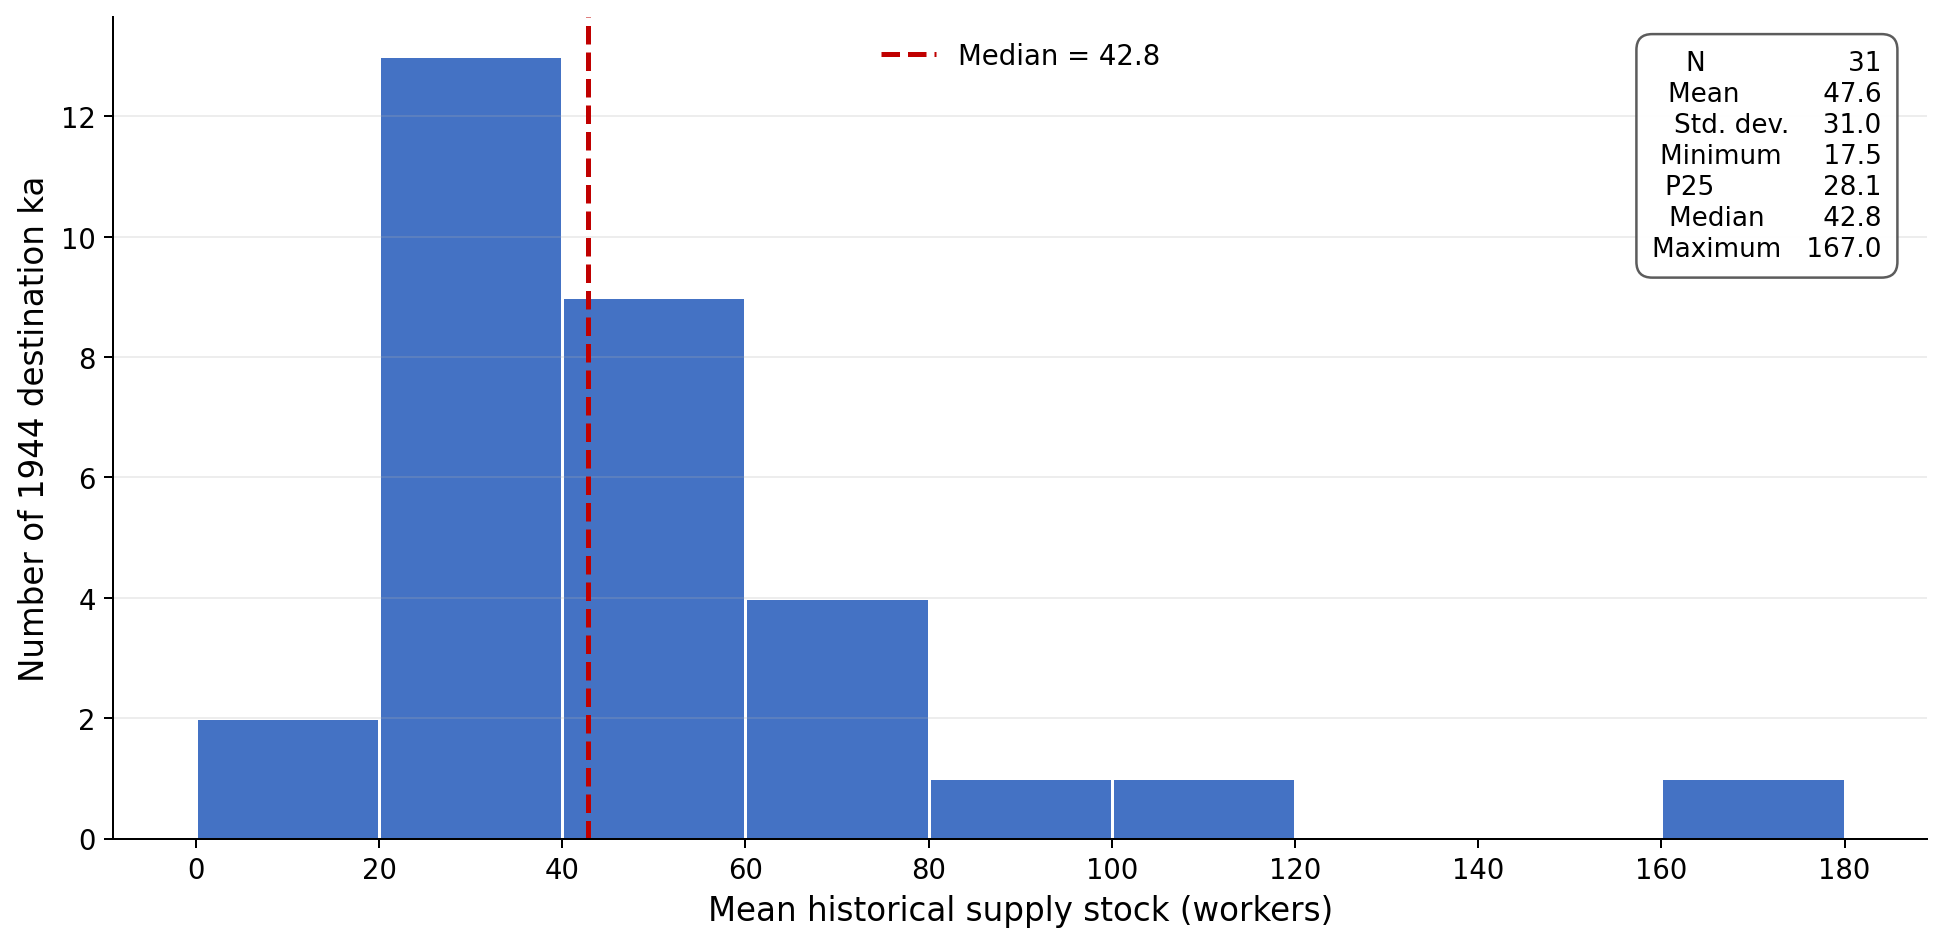
\includegraphics[width=0.98\textwidth,height=0.79\textheight,keepaspectratio]{supply_stock_histogram.png}
\vspace{-0.4em}\raggedright
{\tiny \textit{Notes:} Distribution across 31 unique 1944 ka names with at least one drafted man and positive historical stock. Stock is the mean annual count across all mapped 1938--1943 Tokyo Fu and Tokyo Shi predecessor offices. Duplicate ka names across bureaus are averaged by normalized ka name.}
\end{frame}
\end{document}
